\chapter{Экспериментальная часть}

Для формирования системы запросов о крепости пива, возникла необходимость провести опрос среди респондентов и построить функцию принадлежности термам числовых значений признака, описываемого лингвистической переменной.

В данном разделе приведена анкета, отправленная респондентам. Также представлены результаты анкетирования и статистической обработки мнений респондентов.

\section{Анкета для респондентов}
В таблице \ref{tbl:1} представлена таблица-анкета, предоставленная респондентам.

\begin{table}[H]
	\caption{Анкета, предоставленная респондентам}
	\label{tbl:1}
	\begin{center}
	\begin{tabular}{|c|c|ccccccc|}
		\cline{1-9}
		&                            & \multicolumn{7}{c|}{Крепость пива $\xi$, градусов}                                                                                                    \\ \cline{3-9}
		\multirow{-2}{*}{\begin{tabular}[c]{@{}c@{}}Ид. респ.\end{tabular}} & \multirow{-2}{*}{Терм $i$} & \multicolumn{1}{c|}{0} & \multicolumn{1}{c|}{1} & \multicolumn{1}{c|}{3} & \multicolumn{1}{c|}{5} & \multicolumn{1}{c|}{7} & \multicolumn{1}{c|}{9} & \multicolumn{1}{c|}{11} \\ \cline{1-9}
		{\color[HTML]{333333} }                                                 & безалкогольное                  & \multicolumn{1}{c|}{}  & \multicolumn{1}{c|}{}     & \multicolumn{1}{c|}{}      & \multicolumn{1}{c|}{}       & \multicolumn{1}{c|}{}       &         \multicolumn{1}{c|}{} & \multicolumn{1}{c|}{}    \\ \cline{2-9}
		{\color[HTML]{333333} }                                                 & некрепкое            & \multicolumn{1}{c|}{}  & \multicolumn{1}{c|}{}     & \multicolumn{1}{c|}{}      & \multicolumn{1}{c|}{}       & \multicolumn{1}{c|}{}       &    \multicolumn{1}{c|}{}  & \multicolumn{1}{c|}{}  \\ \cline{2-9}
		{\color[HTML]{333333} }                                                 & слабое            & \multicolumn{1}{c|}{}  & \multicolumn{1}{c|}{}     & \multicolumn{1}{c|}{}      & \multicolumn{1}{c|}{}       & \multicolumn{1}{c|}{}       &   \multicolumn{1}{c|}{}   & \multicolumn{1}{c|}{} \\ \cline{2-9}
		{\color[HTML]{333333} }                                                 & нормальное                     & \multicolumn{1}{c|}{}  & \multicolumn{1}{c|}{}     & \multicolumn{1}{c|}{}      & \multicolumn{1}{c|}{}       & \multicolumn{1}{c|}{}       &   \multicolumn{1}{c|}{}   & \multicolumn{1}{c|}{} \\ \cline{2-9}
		{\color[HTML]{333333} }                                                 & крепкое              & \multicolumn{1}{c|}{}  & \multicolumn{1}{c|}{}     & \multicolumn{1}{c|}{}      & \multicolumn{1}{c|}{}       & \multicolumn{1}{c|}{}       &   \multicolumn{1}{c|}{}  & \multicolumn{1}{c|}{} \\ \cline{2-9}
		\multirow{-6}{*}{{\color[HTML]{333333} 1}}                              & очень крепкое         & \multicolumn{1}{c|}{}  & \multicolumn{1}{c|}{}     & \multicolumn{1}{c|}{}      & \multicolumn{1}{c|}{}       & \multicolumn{1}{c|}{}       &   \multicolumn{1}{c|}{}   & \multicolumn{1}{c|}{} \\ \cline{1-9}
	\end{tabular}
	\end{center}
\end{table}

\section{Результаты анкетирования}
В таблице \ref{tbl:2} представлено соответствие идентификаторов анкетируемых их фамилиям. Респондентами выступали сокомандники в рамках практикума по курсу <<Архитектура ЭВМ>>.

В таблице \ref{tbl:3} представлены результаты анкетирования.

\begin{table}[H]
	\begin{center}
	\caption{Соответствие идентификатора респондента и респондента}
	\label{tbl:2}
	\begin{tabular}{|c|c|}
		\hline
		Ид.  & Респондент      \\ \hline
		1              & Карпова~Е.~О.    \\ \hline
		2              & Глотов~И.~А.   \\ \hline
		3              & Ляпина~Н.~В.    \\ \hline
		4              & Аскарян~К.~А.   \\ \hline
		5              & Обревская~В.~В. \\ \hline
	\end{tabular}
	\end{center}
\end{table}

\begin{table}[H]
	\caption{Результаты анкетирования респондентов}
	\label{tbl:3}
	\begin{center}
	\begin{tabular}{|c|c|ccccccc|}
		\cline{1-9}
		&                                           & \multicolumn{7}{c|}{Крепость пива $\xi$, градусов}                                                                                                                                              \\ \cline{3-9}
		\multirow{-2}{*}{\begin{tabular}[c]{@{}c@{}}Ид. респ.\end{tabular}} & \multirow{-2}{*}{Терм $i$}                & \multicolumn{1}{c|}{0}          & \multicolumn{1}{c|}{1}              & \multicolumn{1}{c|}{3}                     & \multicolumn{1}{c|}{5} & \multicolumn{1}{c|}{7} & \multicolumn{1}{c|}{9} & \multicolumn{1}{c|}{11} \\ \cline{1-9}
		{\color[HTML]{333333} }                                                    & безалкогольное                                 
		& \multicolumn{1}{c|}{1}                        
		& \multicolumn{1}{c|}{1}                        
		& \multicolumn{1}{c|}{0}     
		& \multicolumn{1}{c|}{0}      
		& \multicolumn{1}{c|}{0}      
		& \multicolumn{1}{c|}{0}        
		& \multicolumn{1}{c|}{0} \\ \cline{2-9}
		{\color[HTML]{333333} }                                                    & некрепкое                           
		& \multicolumn{1}{c|}{{\color[HTML]{333333} 0}} 
		& \multicolumn{1}{c|}{{\color[HTML]{333333} 0}} & \multicolumn{1}{c|}{1}     
		& \multicolumn{1}{c|}{0}      
		& \multicolumn{1}{c|}{0}      
		& \multicolumn{1}{c|}{0}        
		& \multicolumn{1}{c|}{0}  \\ \cline{2-9}
		{\color[HTML]{333333} }                                                    & слабое                           
		& \multicolumn{1}{c|}{{\color[HTML]{333333} 0}} 
		& \multicolumn{1}{c|}{{\color[HTML]{333333} 0}} 
		& \multicolumn{1}{c|}{0}     
		& \multicolumn{1}{c|}{1}      
		& \multicolumn{1}{c|}{0}      
		& \multicolumn{1}{c|}{0}       
		& \multicolumn{1}{c|}{0}  \\ \cline{2-9}
		{\color[HTML]{333333} }                                                    & нормальное                                    
		& \multicolumn{1}{c|}{{\color[HTML]{333333} 0}} 
		& \multicolumn{1}{c|}{{\color[HTML]{333333} 0}} 
		& \multicolumn{1}{c|}{0}     
		& \multicolumn{1}{c|}{0}      
		& \multicolumn{1}{c|}{1}      
		& \multicolumn{1}{c|}{1}        
		& \multicolumn{1}{c|}{0}  \\ \cline{2-9}
		{\color[HTML]{333333} }                                                    & крепкое                              
		& \multicolumn{1}{c|}{{\color[HTML]{333333} 0}} 
		& \multicolumn{1}{c|}{{\color[HTML]{333333} 0}} 
		& \multicolumn{1}{c|}{0}     
		& \multicolumn{1}{c|}{0}      
		& \multicolumn{1}{c|}{0}      
		& \multicolumn{1}{c|}{0}        
		& \multicolumn{1}{c|}{0}  \\ \cline{2-9}
		\multirow{-6}{*}{{\color[HTML]{333333} 1}}                                 & очень крепкое                       
		& \multicolumn{1}{c|}{{\color[HTML]{333333} 0}} 
		& \multicolumn{1}{c|}{{\color[HTML]{333333} 0}} 
		& \multicolumn{1}{c|}{0}     
		& \multicolumn{1}{c|}{0}      
		& \multicolumn{1}{c|}{0}      
		& \multicolumn{1}{c|}{0}        
		& \multicolumn{1}{c|}{1}  \\ \cline{1-9}
		{\color[HTML]{333333} }                                                    & безалкогольное                                 
		& \multicolumn{1}{c|}{1}                        
		& \multicolumn{1}{c|}{0}                        
		& \multicolumn{1}{c|}{0}     
		& \multicolumn{1}{c|}{0}      
		& \multicolumn{1}{c|}{0}      
		& \multicolumn{1}{c|}{0}        
		& \multicolumn{1}{c|}{0}  \\ \cline{2-9}
		{\color[HTML]{333333} }                                                    & некрепкое                           
		& \multicolumn{1}{c|}{{\color[HTML]{333333} 0}} 
		& \multicolumn{1}{c|}{{\color[HTML]{333333} 1}} 
		& \multicolumn{1}{c|}{0}    
		 & \multicolumn{1}{c|}{0}     
		  & \multicolumn{1}{c|}{0}     
		   & \multicolumn{1}{c|}{0}        &      \multicolumn{1}{c|}{0}                 \\ \cline{2-9}
		{\color[HTML]{333333} }                                                    & слабое                          
		 & \multicolumn{1}{c|}{{\color[HTML]{333333} 0}} 
		 & \multicolumn{1}{c|}{{\color[HTML]{333333} 0}} 
		 & \multicolumn{1}{c|}{0}     
		 & \multicolumn{1}{c|}{0}      
		 & \multicolumn{1}{c|}{0}      
		 & \multicolumn{1}{c|}{0}       
		  &            \multicolumn{1}{c|}{0}           \\ \cline{2-9}
		{\color[HTML]{333333} }                                                    & нормальное                                    
		& \multicolumn{1}{c|}{{\color[HTML]{333333} 0}} 
		& \multicolumn{1}{c|}{{\color[HTML]{333333} 0}} 
		& \multicolumn{1}{c|}{1}    
		 & \multicolumn{1}{c|}{1}      
		 & \multicolumn{1}{c|}{0}      
		 & \multicolumn{1}{c|}{0}       
		  & \multicolumn{1}{c|}{0}                       \\ \cline{2-9}
		{\color[HTML]{333333} }                                                    & крепкое                              
		& \multicolumn{1}{c|}{{\color[HTML]{333333} 0}} 
		& \multicolumn{1}{c|}{{\color[HTML]{333333} 0}} 
		& \multicolumn{1}{c|}{0}     
		& \multicolumn{1}{c|}{0}      
		& \multicolumn{1}{c|}{1}      
		& \multicolumn{1}{c|}{1}        
		& \multicolumn{1}{c|}{0}                       \\ \cline{2-9}
		\multirow{-6}{*}{{\color[HTML]{333333} 2}}                                 & очень крепкое                        
		& \multicolumn{1}{c|}{{\color[HTML]{333333} 0}} 
		& \multicolumn{1}{c|}{{\color[HTML]{333333} 0}} 
		& \multicolumn{1}{c|}{0}     
		& \multicolumn{1}{c|}{0}      
		& \multicolumn{1}{c|}{0}      
		& \multicolumn{1}{c|}{0}        
		& \multicolumn{1}{c|}{1}                       \\ \cline{1-9}
		
		
		{\color[HTML]{333333} }                                                    & безалкогольное                                 & \multicolumn{1}{c|}{1}                        & \multicolumn{1}{c|}{0}                        & \multicolumn{1}{c|}{0}     & \multicolumn{1}{c|}{0}      & \multicolumn{1}{c|}{0}      & \multicolumn{1}{c|}{0}        & \multicolumn{1}{c|}{0}  \\ \cline{2-9}
		{\color[HTML]{333333} }                                                    & {\color[HTML]{333333} некрепкое}    & \multicolumn{1}{c|}{{\color[HTML]{333333} 0}} & \multicolumn{1}{c|}{{\color[HTML]{333333} 1}} & \multicolumn{1}{c|}{1}     & \multicolumn{1}{c|}{0}      & \multicolumn{1}{c|}{0}      & \multicolumn{1}{c|}{0}        & \multicolumn{1}{c|}{0}                       \\ \cline{2-9}
		{\color[HTML]{333333} }                                                    & {\color[HTML]{333333} слабое}    & \multicolumn{1}{c|}{{\color[HTML]{333333} 0}} & \multicolumn{1}{c|}{{\color[HTML]{333333} 0}} & \multicolumn{1}{c|}{0}     & \multicolumn{1}{c|}{0}      & \multicolumn{1}{c|}{0}      & \multicolumn{1}{c|}{0}        & \multicolumn{1}{c|}{0}                       \\ \cline{2-9}
		{\color[HTML]{333333} }                                                    & {\color[HTML]{333333} нормальное}             & \multicolumn{1}{c|}{{\color[HTML]{333333} 0}} & \multicolumn{1}{c|}{{\color[HTML]{333333} 0}} & \multicolumn{1}{c|}{0}     & \multicolumn{1}{c|}{1}      & \multicolumn{1}{c|}{0}      & \multicolumn{1}{c|}{0}        & \multicolumn{1}{c|}{0}                       \\ \cline{2-9}
		{\color[HTML]{333333} }                                                    & {\color[HTML]{333333} крепкое}       & \multicolumn{1}{c|}{{\color[HTML]{333333} 0}} & \multicolumn{1}{c|}{{\color[HTML]{333333} 0}} & \multicolumn{1}{c|}{0}     & \multicolumn{1}{c|}{0}      & \multicolumn{1}{c|}{0}      & \multicolumn{1}{c|}{0}        & \multicolumn{1}{c|}{0}                       \\ \cline{2-9}
		\multirow{-6}{*}{{\color[HTML]{333333} 3}}                                 & {\color[HTML]{333333} очень крепкое  } & \multicolumn{1}{c|}{{\color[HTML]{333333} 0}} & \multicolumn{1}{c|}{{\color[HTML]{333333} 0}} & \multicolumn{1}{c|}{0}     & \multicolumn{1}{c|}{0}      & \multicolumn{1}{c|}{1}      & \multicolumn{1}{c|}{1}        & \multicolumn{1}{c|}{1}                       \\ \cline{1-9}
		{\color[HTML]{333333} }                                                    & безалкогольное                                 & \multicolumn{1}{c|}{1}                        & \multicolumn{1}{c|}{1}                        & \multicolumn{1}{c|}{0}     & \multicolumn{1}{c|}{0}      & \multicolumn{1}{c|}{0}      & \multicolumn{1}{c|}{0}        & \multicolumn{1}{c|}{0}  \\ \cline{2-9}
		{\color[HTML]{333333} }                                                    & {\color[HTML]{333333} некрепкое}    & \multicolumn{1}{c|}{{\color[HTML]{333333} 0}} & \multicolumn{1}{c|}{{\color[HTML]{333333} 0}} & \multicolumn{1}{c|}{1}     & \multicolumn{1}{c|}{0}      & \multicolumn{1}{c|}{0}      & \multicolumn{1}{c|}{0}        & \multicolumn{1}{c|}{0}                       \\ \cline{2-9}
		{\color[HTML]{333333} }                                                    & {\color[HTML]{333333} слабое}    & \multicolumn{1}{c|}{{\color[HTML]{333333} 0}} & \multicolumn{1}{c|}{{\color[HTML]{333333} 0}} & \multicolumn{1}{c|}{0}     & \multicolumn{1}{c|}{1}   & \multicolumn{1}{c|}{0}      & \multicolumn{1}{c|}{0}        & \multicolumn{1}{c|}{0}                       \\ \cline{2-9}
		{\color[HTML]{333333} }                                                    & {\color[HTML]{333333} нормальное}             & \multicolumn{1}{c|}{{\color[HTML]{333333} 0}} & \multicolumn{1}{c|}{{\color[HTML]{333333} 0}} & \multicolumn{1}{c|}{0}     & \multicolumn{1}{c|}{0}      & \multicolumn{1}{c|}{1}      & \multicolumn{1}{c|}{0}        & \multicolumn{1}{c|}{0}                       \\ \cline{2-9}
		{\color[HTML]{333333} }                                                    & {\color[HTML]{333333} крепкое}       & \multicolumn{1}{c|}{{\color[HTML]{333333} 0}} & \multicolumn{1}{c|}{{\color[HTML]{333333} 0}} & \multicolumn{1}{c|}{0}     & \multicolumn{1}{c|}{0}      & \multicolumn{1}{c|}{0}      & \multicolumn{1}{c|}{1}        & \multicolumn{1}{c|}{0}                       \\ \cline{2-9}
		\multirow{-6}{*}{{\color[HTML]{333333} 4}}                                 & {\color[HTML]{333333} очень крепкое  } & \multicolumn{1}{c|}{{\color[HTML]{333333} 0}} & \multicolumn{1}{c|}{{\color[HTML]{333333} 0}} & \multicolumn{1}{c|}{0}     & \multicolumn{1}{c|}{0}      & \multicolumn{1}{c|}{0}      & \multicolumn{1}{c|}{0}        & \multicolumn{1}{c|}{1}                       \\ \cline{1-9}
		{\color[HTML]{333333} }                                                    & безалкогольное                                 & \multicolumn{1}{c|}{1}                        & \multicolumn{1}{c|}{0}                        & \multicolumn{1}{c|}{0}     & \multicolumn{1}{c|}{0}      & \multicolumn{1}{c|}{0}      & \multicolumn{1}{c|}{0}        & \multicolumn{1}{c|}{0}  \\ \cline{2-9}
		{\color[HTML]{333333} }                                                    & {\color[HTML]{333333} некрепкое}    & \multicolumn{1}{c|}{{\color[HTML]{333333} 0}} & \multicolumn{1}{c|}{{\color[HTML]{333333} 1}} & \multicolumn{1}{c|}{0}      & \multicolumn{1}{c|}{0}      & \multicolumn{1}{c|}{0}      & \multicolumn{1}{c|}{0}        & \multicolumn{1}{c|}{0}                       \\ \cline{2-9}
		{\color[HTML]{333333} }                                                    & {\color[HTML]{333333} слабое}    & \multicolumn{1}{c|}{{\color[HTML]{333333} 0}} & \multicolumn{1}{c|}{{\color[HTML]{333333} 0}} & \multicolumn{1}{c|}{1}     & \multicolumn{1}{c|}{1}      & \multicolumn{1}{c|}{0}      & \multicolumn{1}{c|}{0}        & \multicolumn{1}{c|}{0}                       \\ \cline{2-9}
		{\color[HTML]{333333} }                                                    & {\color[HTML]{333333} нормальное}             & \multicolumn{1}{c|}{{\color[HTML]{333333} 0}} & \multicolumn{1}{c|}{{\color[HTML]{333333} 0}} & \multicolumn{1}{c|}{0}     & \multicolumn{1}{c|}{0}      & \multicolumn{1}{c|}{1}      & \multicolumn{1}{c|}{0}        & \multicolumn{1}{c|}{0}                       \\ \cline{2-9}
		{\color[HTML]{333333} }                                                    & {\color[HTML]{333333} крепкое}       & \multicolumn{1}{c|}{{\color[HTML]{333333} 0}} & \multicolumn{1}{c|}{{\color[HTML]{333333} 0}} & \multicolumn{1}{c|}{0}     & \multicolumn{1}{c|}{0}      & \multicolumn{1}{c|}{0}      & \multicolumn{1}{c|}{1}        & \multicolumn{1}{c|}{0}                       \\ \cline{2-9}
		\multirow{-6}{*}{{\color[HTML]{333333} 5}}                                 & {\color[HTML]{333333} очень крепкое  } & \multicolumn{1}{c|}{{\color[HTML]{333333} 0}} & \multicolumn{1}{c|}{{\color[HTML]{333333} 0}} & \multicolumn{1}{c|}{0}     & \multicolumn{1}{c|}{0}      & \multicolumn{1}{c|}{0}      & \multicolumn{1}{c|}{0}        & \multicolumn{1}{c|}{1}                       \\ \cline{1-9}
	\end{tabular}
	\end{center}
\end{table}

\section{Функция принадлежности}
В таблице \ref{tbl:4} представлены значения функции принадлежности термам числовых значений признака, описываемого лингвистической переменной.

\begin{table}[H]
	\begin{center}
	\caption{Таблица значений функции принадлежности}
	\label{tbl:4}
	\begin{tabular}{|c|c|c|c|c|c|c|c|c|c|}
		\cline{1-9}
		\multirow{2}{*}{безалкогольное}          &  $\mu_j(\xi)$ & 5   & 5   & 2   & 0   & 0   & 0   &  0\\ \cline{2-9}
		& $F_j(\xi)$ & 1.0 & 0.4 & 0.0 & 0.0 & 0.0 & 0.0 &  0.0\\ \cline{1-9}
		\multirow{2}{*}{некрепкое}    &  $\mu_j(\xi)$ & 0   & 3   & 3   & 0   & 0   & 0   &  0\\ \cline{2-9}
		& $F_j(\xi)$ & 0.0 & 0.6 & 0.6 & 0.0 & 0.0 & 0.0 & 0.0 \\ \cline{1-9}
		\multirow{2}{*}{слабое}    &  $\mu_j(\xi)$ & 0   & 0   & 1   & 4   & 0   & 0   &  0\\ \cline{2-9}
		& $F_j(\xi)$ & 0.0 & 0.0 & 0.2 & 0.6 & 0.0 & 0.0 & 0.0 \\ \cline{1-9}
		\multirow{2}{*}{нормальное}             &  $\mu_j(\xi)$ & 0   & 0   & 1   & 2   & 3   & 1   & 0 \\ \cline{2-9}
		& $F_j(\xi)$ & 0.0 & 0.0 & 0.0 & 0.2 & 0.4 & 0.6 & 0.2 \\ \cline{1-9}
		\multirow{2}{*}{крепкое}       &  $\mu_j(\xi)$ & 0   & 0   & 0   & 0   & 1  & 3   & 1 \\ \cline{2-9}
		& $F_j(\xi)$ & 0.0 & 0.0 & 0.0 & 0.0 & 0.2 & 0.6 & 0.2 \\ \cline{1-9}
		\multirow{2}{*}{очень крепкое} &  $\mu_j(\xi)$ & 0   & 0   & 0   & 0   & 1   & 1   &  4 \\ \cline{2-9}
		& $F_j(\xi)$ & 0.0 & 0.0 & 0.0 & 0.0 & 0.2 & 0.2 & 0.8 \\ \cline{1-9}
	\end{tabular}
	\end{center}
\end{table}

В таблице используются следующие обозначения:

\begin{itemize}
	\item $\mu_j(\xi) = \sum\limits_{k=1}^N a^{k}_{ji}$;
	\item $F_j(\xi) = \frac{S_j}{N}$,
	\item $N$~---~количество респондентов.
\end{itemize}

\newpage

На рис. \ref{img:1} изображена функциональная зависимость $F_j(\xi)$.

\begin{figure}[h!]
\centering
    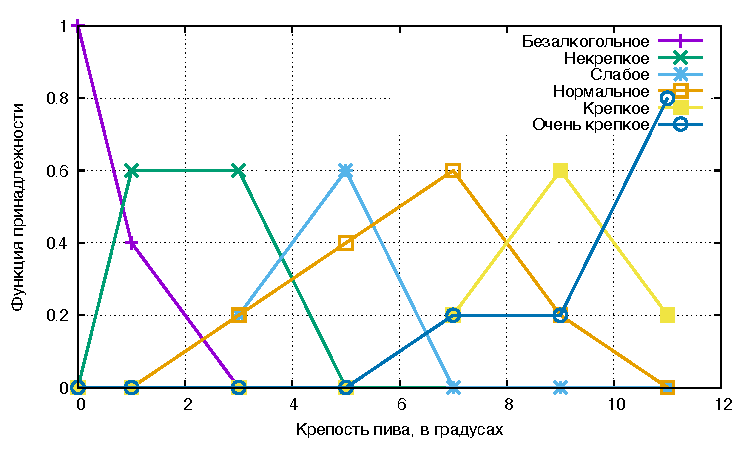
\includegraphics[width=0.8\linewidth]{../data/beer.pdf}
    \caption{Функциональная зависимость}
    \label{img:1}	
\end{figure}

\section{Соответствие признаков и диапазонов значений}
В таблице \ref{tbl:5} представлено соответствие между термами и диапазонами значений для крепости пива в градусах.

\begin{table}[H]
	\begin{center}
	\caption{Соответствие между термами и диапазонами значений для крепости пива в градусах}
	\label{tbl:5}
	\begin{tabular}{|l|l|}
		\hline
		Признак            & Диапазон \\ \hline
		безалкогольное          &  $\left[0.00;0.83\right]$        \\ \hline
		некрепкое    &       $\left[0.83;3.80\right]$    \\ \hline
		слабое    &     $\left[3.80;5.50\right]$      \\ \hline
		нормальное             &    $\left[5.50;8.00\right]$     \\ \hline
		крепкое       &        $\left[8.00;9.80\right]$   \\ \hline
		очень крепкое &    $\left[9.80;11.00\right]$       \\ \hline
	\end{tabular}
	\end{center}
\end{table}



\newpage